\documentclass{beamer}

\usetheme{Darmstadt} % Tema de ejemplo, siéntase libre de elegir otro

\usepackage[spanish]{babel} % Para usar el idioma español

\usepackage{amsmath} % Para ecuaciones matemáticas avanzadas
\usepackage{amsfonts} % Para símbolos matemáticos

\title{Conceptos Elementales de Funciones Armónicas}
% \author{Su Nombre} % Opcional
\date{\today} % Opcional

\begin{document}
% Diapositiva 1: Diapositiva del Título
\begin{frame}
  \titlepage
\end{frame}

% Diapositiva 2: ¿Qué es una Función Armónica?
\begin{frame}
  \frametitle{¿Qué es una Función Armónica?}

  \begin{itemize}
    \item En matemáticas, física y procesos estocásticos, una \textbf{función armónica} es una función $f : U \to \mathbb{R}$ dos veces continuamente diferenciable [1].
    \item El dominio $U$ es un subconjunto abierto de $\mathbb{R}^n$ [1].
    \item Una función es armónica si satisface la \textbf{ecuación de Laplace} en todos los puntos de $U$ [1].
    \item La ecuación de Laplace se expresa como:
      \[ \frac{\partial^2 f}{\partial x_1^2} + \frac{\partial^2 f}{\partial x_2^2} + \cdots + \frac{\partial^2 f}{\partial x_n^2} = 0 \]
      o escrita de forma más compacta como $\nabla^2 f = 0$ o $\Delta f = 0$ .
  \item El término ``armónica'' proviene de la solución de la ecuación diferencial del movimiento armónico en una cuerda tensa, referidos como ``armónicos''. Las funciones que satisfacen la ecuación de Laplace fueron posteriormente referidas como \emph{armónicas}.
  \end{itemize}
\end{frame}

% Diapositiva 3: La Ecuación de Laplace y Propiedades
\begin{frame}
  \frametitle{La Ecuación de Laplace y Propiedades}

  \begin{itemize}
          \small
    \item El conjunto de funciones armónicas en un conjunto abierto $U$ dado forma un \textbf{espacio vectorial sobre $\mathbb{R}$} [3]. Las combinaciones lineales de funciones armónicas también son armónicas [3].
    \item Las funciones armónicas son \textbf{infinitamente diferenciables} en conjuntos abiertos [4].
    \item De hecho, las funciones armónicas son \textbf{analíticas reales}, lo que significa que pueden expresarse localmente como series de potencias [3, 4]. Este es un hecho general sobre operadores elípticos [3].
    \item Todas las derivadas parciales de una función armónica son también funciones armónicas [3]. El operador de Laplace conmuta con el operador de derivada parcial en esta clase de funciones [3].
    \item En muchos aspectos, las funciones armónicas son análogas de las \textbf{funciones holomorfas} en análisis complejo. La parte real o imaginaria de cualquier función holomorfa es una función armónica en $\mathbb{R}^2$.
  \end{itemize}
  \end{frame}

% Diapositiva 4: Aplicaciones y Ejemplos
\begin{frame}
  \frametitle{Aplicaciones y Ejemplos}

  \begin{itemize}
          \small
    \item Las funciones armónicas surgen en la \textbf{física matemática} y la \textbf{teoría de procesos estocásticos} [1, 9].
    \item \textbf{Dos variables}:
    \begin{itemize}
            \small
        \item La parte real o imaginaria de cualquier función holomorfa [7].
        \item Ejemplos incluyen $f(x, y) = e^x \sin y$ y $f(x, y) = \ln(x^2+y^2)$ (en $\mathbb{R}^2 \smallsetminus \{0\}$) [7]. La última puede describir el potencial eléctrico o de gravedad [7].
    \end{itemize}
    \item \textbf{Tres variables}: Ejemplos incluyen $1/r$ (carga puntual unitaria), $x/r^3$ (dipolo dirigido en $x$) y $-\ln(r^2-z^2)$ (línea de densidad de carga unitaria) [10]. (donde $r^2 = x^2+y^2+z^2$) [10].
    \item \textbf{n variables}: Ejemplos incluyen funciones constantes, lineales y afines en todo $\mathbb{R}^n$ [11]. La función $f(x_1, \dots, x_n) = (x_1^2 + \cdots + x_n^2)^{1-n/2}$ en $\mathbb{R}^n \smallsetminus \{0\}$ para $n>2$ también es armónica.
    \item En física, las funciones armónicas están determinadas por sus \textbf{singularidades y condiciones de contorno} [9]. A menudo son proporcionales al potencial electrostático debido a distribuciones de carga.
  \end{itemize}
\end{frame}

% Diapositiva 5: La Propiedad del Valor Medio
\begin{frame}
  \frametitle{La Propiedad del Valor Medio}

  \begin{itemize}
          \small
    \item Una propiedad clave de las funciones armónicas es la \textbf{propiedad del valor medio}.
    \item Si $B(x, r)$ es una bola contenida completamente dentro del dominio $\Omega \subset \mathbb{R}^n$ de una función armónica $u: \Omega \to \mathbb{R}$, entonces el valor de $u$ en el centro $x$ es igual al valor promedio de $u$ en la superficie de la bola.
    \item Este valor promedio también es igual al valor promedio de $u$ en el interior de la bola.
    \item Matemáticamente, para $u$ armónica en $\Omega$ y $B(x,r) \subset \Omega$:
      \[ u(x) = \frac{1}{n\omega_n r^{n-1}}\int_{\partial B(x,r)}u\,d\sigma = \frac{1}{\omega_n r^n}\int_{B(x,r)}u\,dV \]
      donde $\omega_n$ es el volumen de la bola unitaria en $n$ dimensiones [13].
    \item \textbf{Importancia}: Recíprocamente, cualquier función localmente integrable que satisfaga la propiedad del valor medio (del volumen) es tanto infinitamente diferenciable como armónica. Esta propiedad esencialmente caracteriza a las funciones armónicas.
  \end{itemize}
  \end{frame}


  %%%%  FRAME  %%%%
  \begin{frame}
      \frametitle{Discretización de la Prop. del Valor Medio}
      \begin{center}
          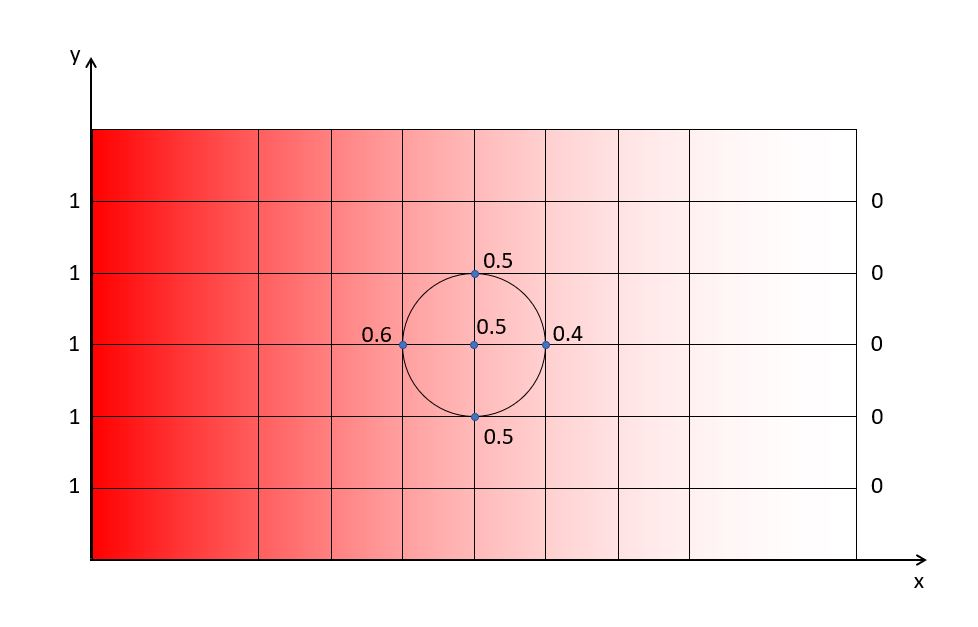
\includegraphics[width=0.9\textwidth]{hot_plate_mean_1.jpg}
      \end{center}
      Crédito: \url{https://rodolphe-vaillant.fr/entry/53/harmonic-function-definitions-and-properties}


  \end{frame}

  \begin{frame}{Discretización de la Ecuación de Laplace}
  \begin{itemize}
          \small
    \item Comenzamos con la \textbf{Ecuación de Laplace estacionaria en 2D} para la temperatura \( T(x,y) \):
    $$ \frac{\partial^2 T}{\partial x^2} + \frac{\partial^2 T}{\partial y^2}=0 $$ 

\item Utilizamos el método de \textbf{diferencias finitas centrales} para las segundas derivadas parciales.
    \item Asumimos un tamaño de malla uniforme: \( \Delta x = \Delta y = h \) [3].
    \item La discretización de \( \frac{\partial^2 T}{\partial x^2} \) en el punto \((i,j)\) es \( \frac{T_{i+1,j}-2T_{i,j}+T_{i-1,j}}{h^2} \).
    \item La discretización de \( \frac{\partial^2 T}{\partial y^2} \) en el punto \((i,j)\) es \( \frac{T_{i,j+1}-2T_{i,j}+T_{i,j-1}}{h^2} \).
    \item Sustituyendo en la Ecuación de Laplace y multiplicando por \( h^2 \), obtenemos la versión discreta:
    $$ T_{i+1,j}+T_{i-1,j}+T_{i,j+1}+T_{i,j-1}-4 T_{i,j}=0 $$
  \end{itemize}
\end{frame}

% Slide 3: 5-Point Formula
\begin{frame}{La Fórmula de 5 Puntos}
  \begin{itemize}
          \small
    \item La ecuación discreta anterior \( T_{i+1,j}+T_{i-1,j}+T_{i,j+1}+T_{i,j-1}-4 T_{i,j}=0 \) [4] es conocida como la \textbf{fórmula de 5 puntos} [5].


    \item Reescribiendo la ecuación con la notación n, s, e, w:
    $$ T_{e}+T_{w}+T_{n}+T_{s}-4 T_{m}=0 $$ 

    \item Finalmente, al despejar \( T_m \), obtenemos la \textbf{Ecuación (6.21)} [7]:
    $$ \mathbf{T_{m}= \frac{T_{e}+T_{w}+T_{n}+T_{s}}{4}} $$ 

    \item Esto significa que la temperatura en el punto central es el \textbf{promedio de las temperaturas de sus cuatro vecinos}.
  \end{itemize}
\end{frame}

\begin{frame}{La Fórmula de 5 Puntos}
    \begin{columns}
        \begin{column}{0.5\textwidth}
            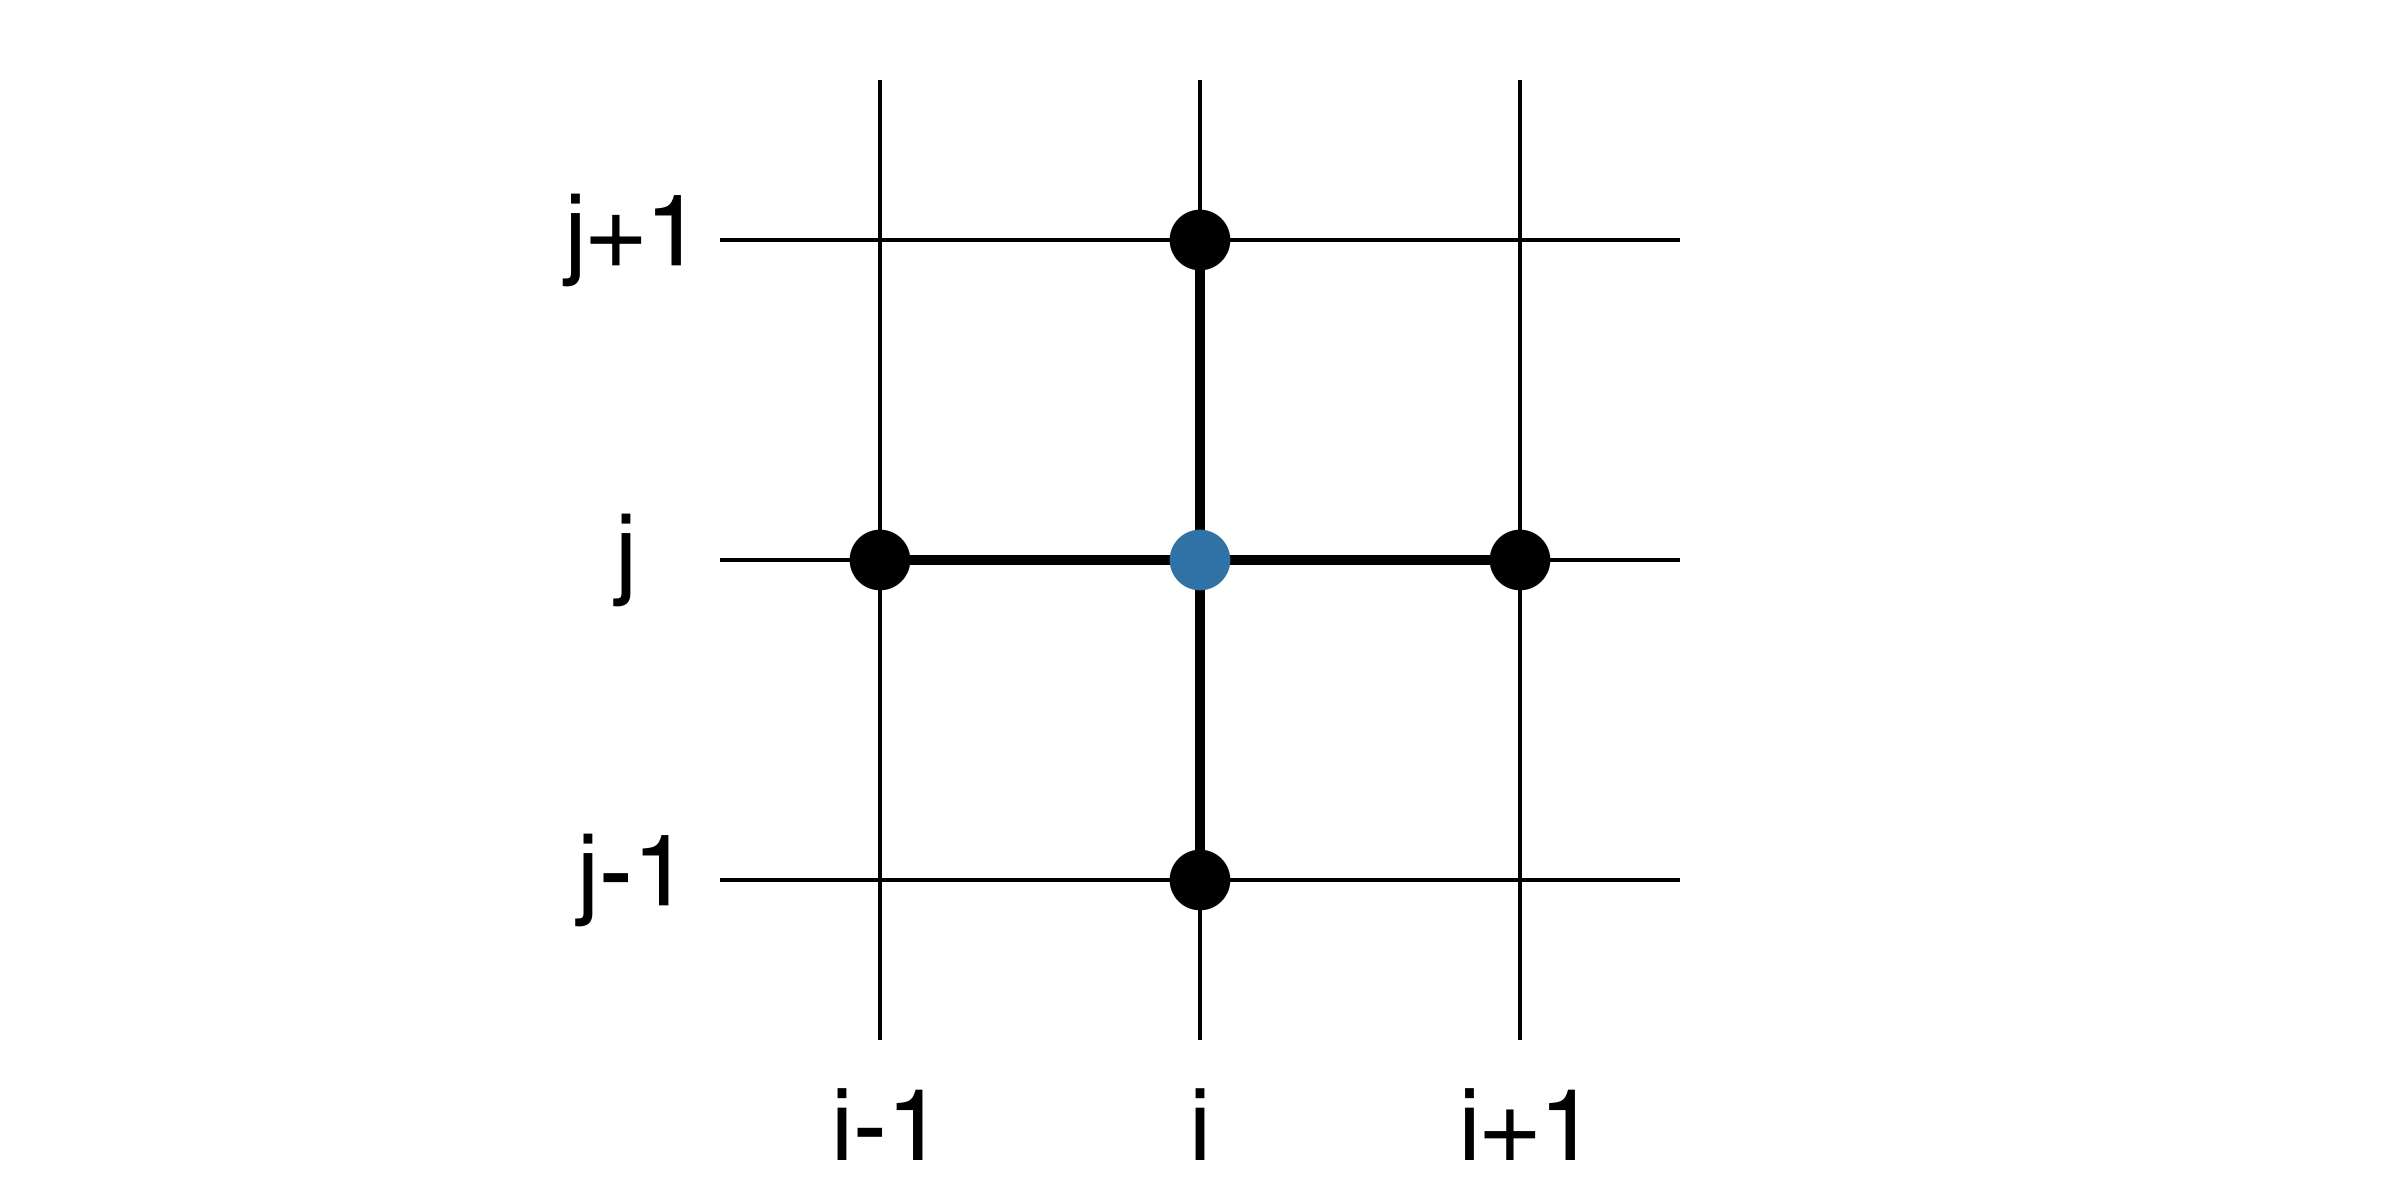
\includegraphics[width=1.3\textwidth]{3.png}
        \end{column}
        \begin{column}{0.5\textwidth}
            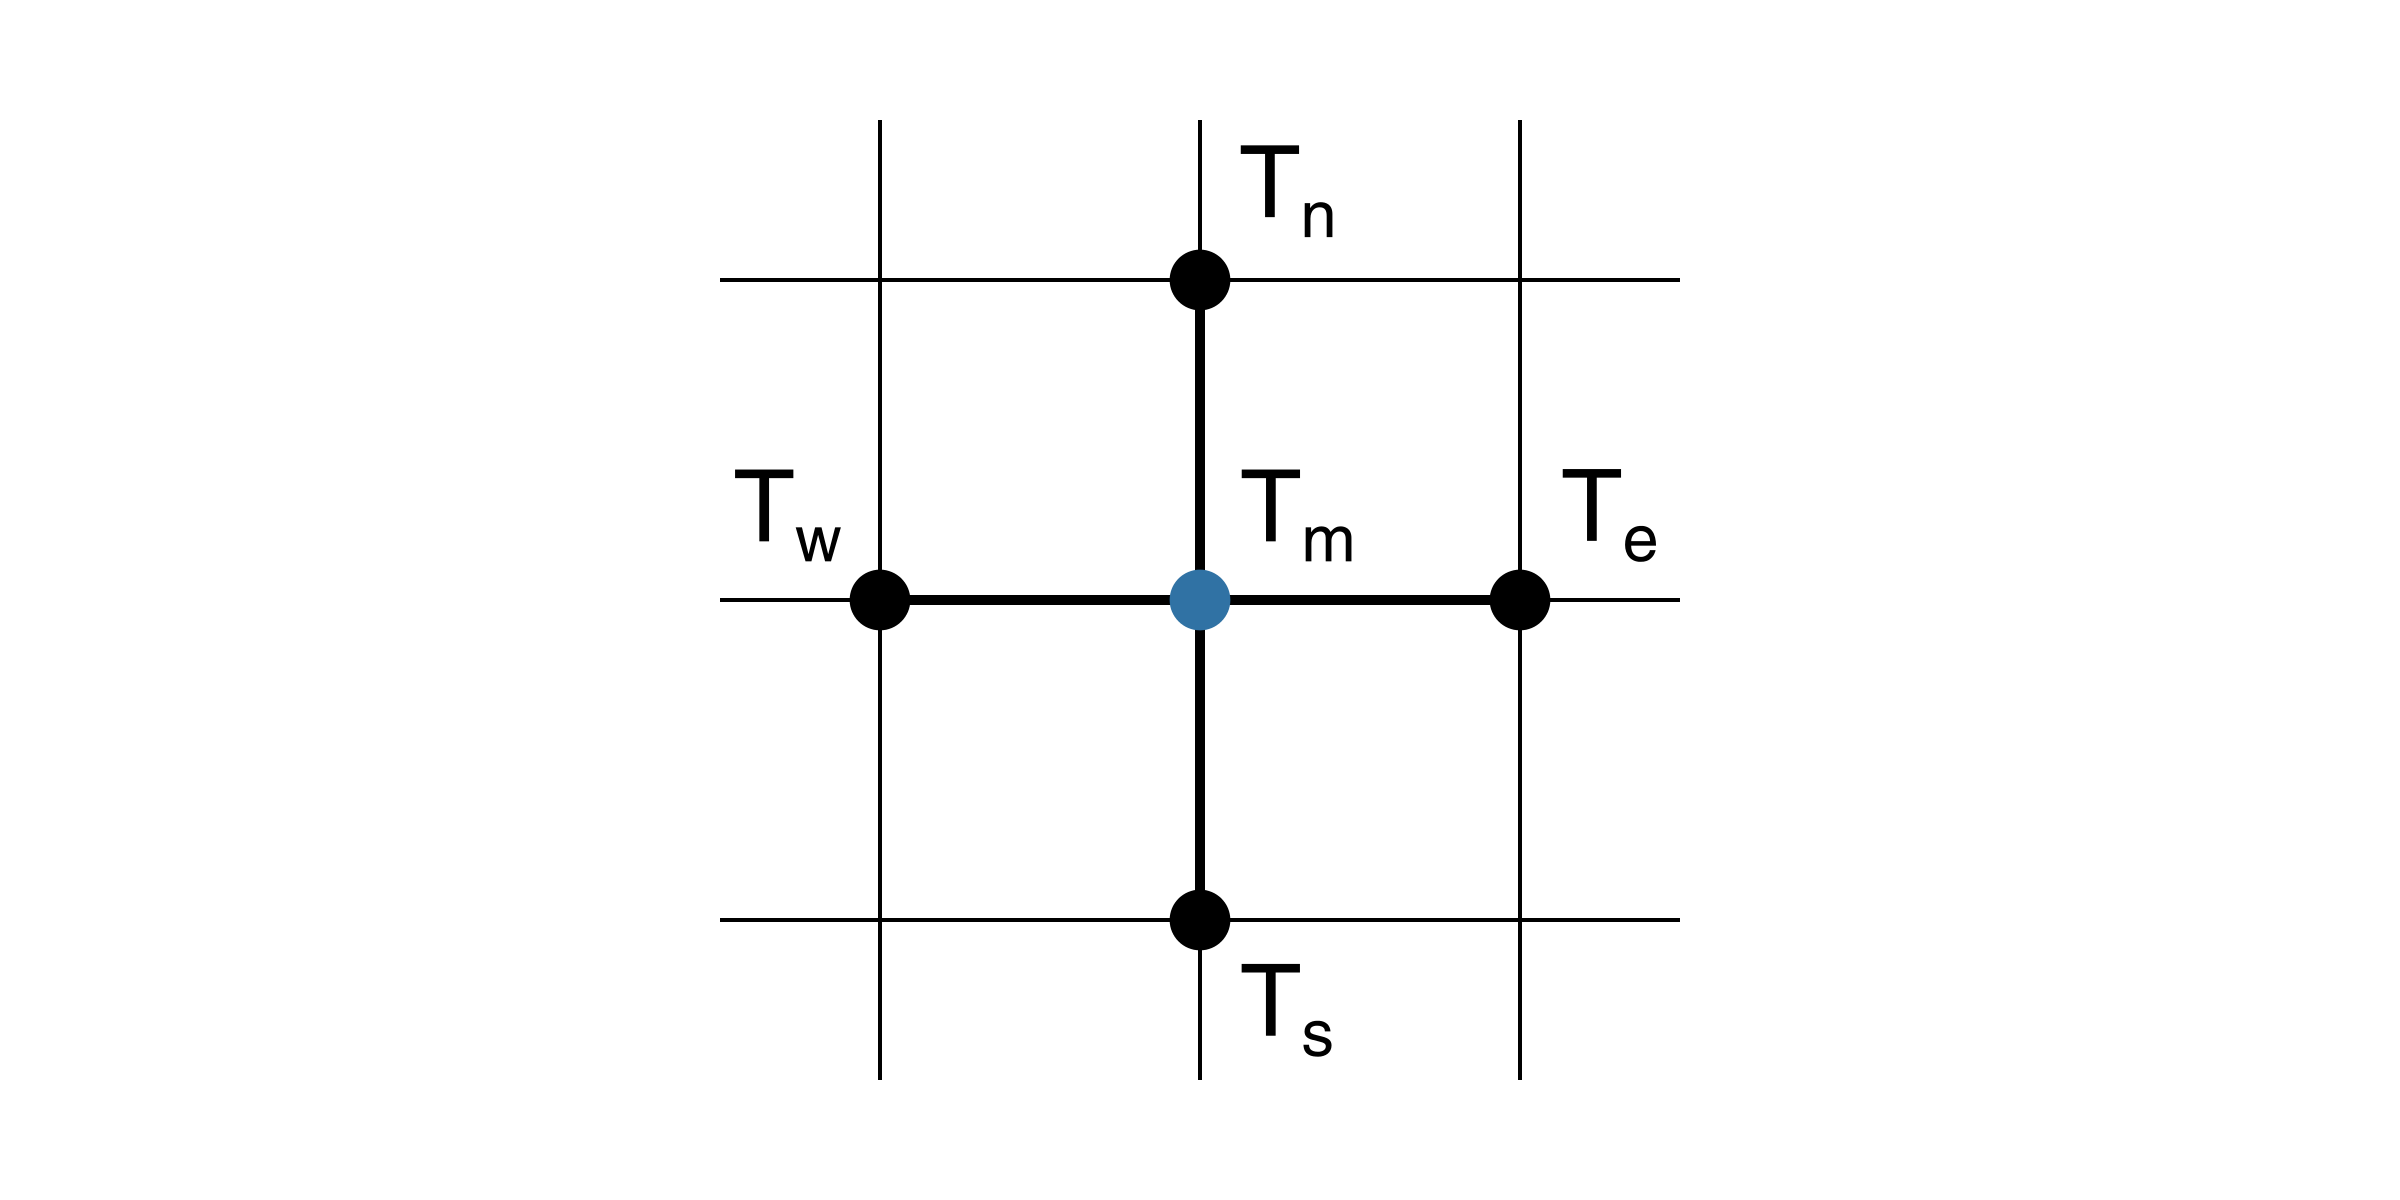
\includegraphics[width=1.3\textwidth]{3_compass.png}
        \end{column}
    \end{columns}
\end{frame}
\end{document}
